\section{Comparison}

\begin{figure*}[b!]
\caption{Comparison of the most important criterias.}
\centering
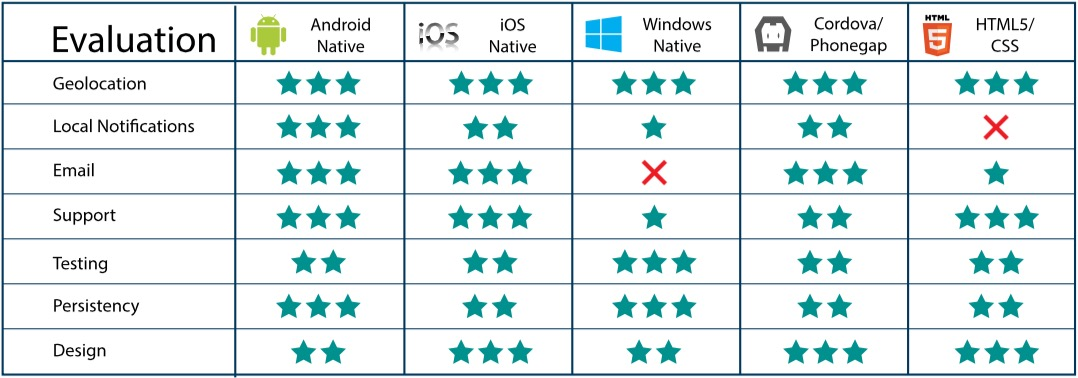
\includegraphics[scale=0.4]{resources/comparison.jpg}
\label{comparison}
\end{figure*}

Figure \ref{comparison} zeigt eine Gegenüberstellung der erreichten Punktzahlen der einzelnen Technologien. Während Android, iOS und Phonegap alle Probleme mit sehr hoher Punktzahl lösen könnten, gab es bei Windows und HTML5 des Öfteren schlechte Bewertungen und es gab sogar Features, die nicht umgesetzt werden konnten. Sowohl HTML5 bräuchte für lokale Notifications Backend-Unterstützung, als auch Windows beim Versenden von Emails mit Anhängen.

Bei der Nutzung von Geolocations und Ortungsdiensten haben alle Technologien die maximale Punktzahl erreicht, somit sind Anforderungen diesbezüglich für keine der Technologien ein K.O. Kriterium.

Im Bezug auf das Design haben die hybriden web-basierten Anwendungen die Nase vorn, wenn es um die Etablierung eines eigenen Designs geht. Sollen die Apps möglichst nativ aussehen, dann könnte es hier etwas aufwändiger werden und der Vorteil, dass bei Phonegap nur eine einzige App implementiert werden muss evtl. wegfallen. IOS ist vom Design her sehr schnell umsetzbar, sofern nur auf die Standard-Widgets zugegriffen wird. 

